% controlled fusion and RF heating and current drive
%\chaptertoc{}

\chapter{Controlled Fusion, RF heating and Current Drive}
\label{chap:fusion_and_rf}
\margintoc

%%%%%%%%%%%%%%%%%%%%%%%%%%%%%%%%%%%%%%%%%%
%%%%%%%%%%%%%%%%%%%%%%%%%%%%%%%%%%%%%%%%%%
\section{Nuclear Fusion}
Nuclear fusion is the process that powers all the stars in the Universe, including our Sun. To get nuclear fusion, nuclei have to come close enough to each other where nuclear forces can overcome their mutual electrostatic repulsion. This would require temperatures of the order of 720 keV for head-on collisions of thermal particles to lead to fusion reactions in a classical way. 

Actually, quantum physics has to be taken into account in the process. Both in tokamaks and in stars interiors, fusion reactions take place predominantly due to the tunnel effect. Crossing this barrier can be quantified in a probabilistic manner with the reaction rate $R$ $[\mathrm{reaction/m^3 s}]$, defined as the probability of reaction per unit time and volume. 
The reaction rate between mono-energetic ions of density $n_1$ $[\si{m}^{-3}]$ striking target ions of density $n_2$ $[\si{m}^{-3}]$ is proportional to the effective cross-section area $\sigma$ $[\si{m}^2]$ and to the velocity difference $v_{12}$ between the two species:
\begin{equation*}
	r_{12} = n_1 n_2 \; \sigma v_{12}
\end{equation*}
The quantity  $\sigma v_{12}$, which depends on the kinetic energy of the colliding particles, is called the reactivity ($\mathrm{[m^3/s]}$). The reaction rate $r_{12}$ is proportional to the square of the density of the mixture. In fusion plasmas, ions are not mono-energetic. They are assumed to have Maxwellian velocity distributions. The average reactivity $\langle \sigma v \rangle_{12}$ derives from the following expression:
\begin{equation*}
	\left < \sigma v \right >_{12} 
	= \int_{-\infty}^{+\infty} \int_{-\infty}^{+\infty} 
	\sigma(v_{12}) v_{12}\;  f_1(v_1) f_2(v_2) \; dv_1dv_2
\end{equation*}

Finally, the average reaction rate $R_{12}$ reads:
\begin{equation*}
	R_{12} = n_1 n_2 \; \left < \sigma v \right >_{12}
\end{equation*}
It governs the time evolution of both densities: $\dv{n_1}{t} = \dv{n_2}{t} = - R_{12}$. The temperature dependence of the reactivity $\langle \sigma v \rangle_{12}$ is plotted on figure \ref{fig:chap1:reactivity} for several fusion reactions.

\begin{figure} 
	\begin{center}
		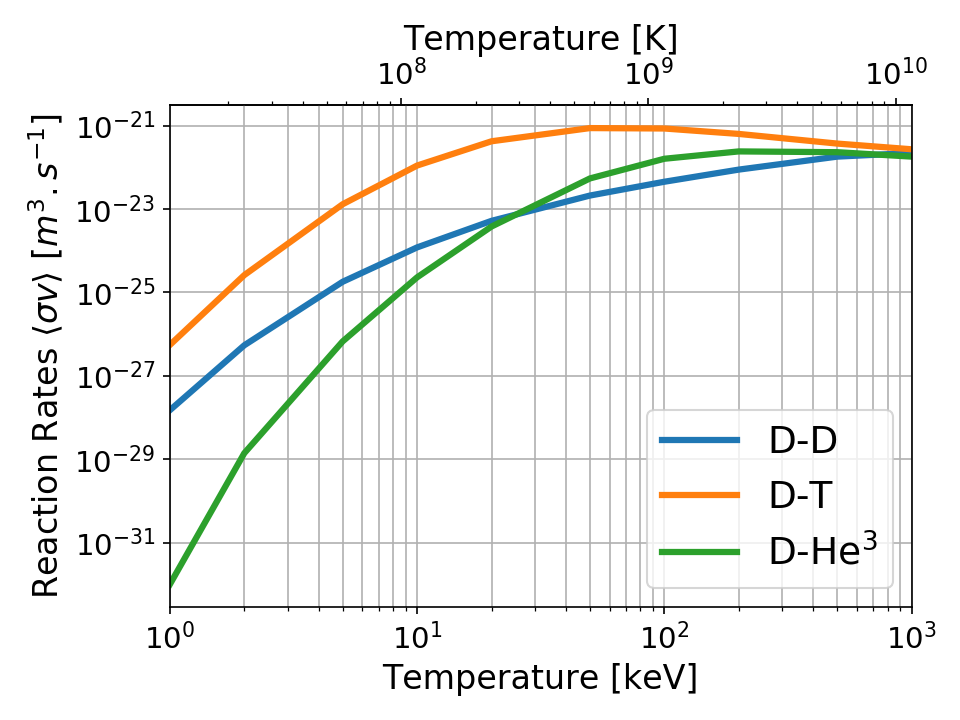
\includegraphics[width=1.0\textwidth]{figures/chap1/Fusion_Reactivity.png}
		\caption{Fusion reactivity versus temperature for few couples of fusion reactions. Data from \citeauthyear{richardson2019}.}
		\label{fig:chap1:reactivity}
	\end{center}
\end{figure}

The D-T reactivity reaches its maximum for a temperature of 64 keV, corresponding to a temperature of $742\,10^6$ K. Since it has the highest reaction rate, the D-T reaction is the “easiest” to initiate (maximum reactivity at lowest temperature) of all fusion reactions and is the main targeted reaction for controlled fusion reactors\sidecite{cea1987, ball2019}: 
\begin{equation}
	\mathrm{D + T} \longrightarrow \mathrm{{}^4 He~(3.56~MeV) + n~(14.03~MeV)}
\end{equation}
Therefore, the D-T reaction leads to a total released energy of $E_{DT}$ = 17.59 \si{MeV} = $2.82\times 10^{-12} \si{J}$ per fusion reaction\sidenote{This value can be compared to the 200~MeV released by $^{235}$U fission. Yet, the energy release \emph{per nucleon} ($i.e.$ per kilogram) is approximately 4 times larger for fusion than for fission reactions.}.

The fusion power per unit volume $p_{DT}$ produced by the fusion of the nuclei of deuterium and tritium reads: 
\begin{equation*}
	P_{fus} = n_D n_T \left< \sigma v \right>_{DT} E_{DT}
\end{equation*}
with $n_D$ and $n_T$ the deuterium and tritium density and $\left< \sigma v \right>_{DT}$ the D-T reactivity. 


The fusion power per unit volume $p_{DT}$ produced by the fusion of the nuclei of deuterium and tritium reads: 
\begin{equation*}
p_{DT} = n_D n_T \left< \sigma v \right>_{DT} E_{DT}
\end{equation*}
with $n_D$ and $n_T$ the deuterium and tritium density and $\left< \sigma v \right>_{DT}$ the D-T reactivity. Assuming equal deuterium and tritium densities:
\begin{equation*}
n_D = n_T = \frac{n}{2}
\end{equation*}
with $n$ the electron density, then the thermonuclear power density is:
\begin{equation*}
p_{DT} = \frac{1}{4} n^2 \left< \sigma v \right>_{DT} E_{DT}
\end{equation*}

%Assuming a constant reactivity in the plasma ("flat profile hypothesis") and using the tore volume $V$, the fusion power is: 
%\begin{equation}
%P_{fus} = \frac{V}{4}
%n^2 \left< \sigma v \right>_{DT} E_{DT}
%\end{equation}
%
%For a circular cross-section, the plasma volume is $V=2\pi^2 R a^2$. The reactivity $\left< \sigma v \right>_{DT}$ depends on the temperature. In the temperature range 10.3-18.5 keV, it turns out that the reactivity $\left< \sigma v \right>_{DT}$ can well (with about 10$\%$ error) be approximated by \sidecite{wesson2011}: 
%\begin{equation*}
%	\left< \sigma v \right>_{DT} \approx 1.18\, 10^{-24}\; \hat T^2 \;\si{\left[m^3 s^{-1}\right]}
%\end{equation*}
%where $\hat T$ is expressed in $\si{keV}$.

%%%%%%%%%%%%%%%%%%%%%%%%%%%%%%%%%%%%%%%%%%
\section{Magnetic Controlled Fusion}
If controlled in a reactor, fusion power could be an ideal energy source. It would run on hydrogen isotopes\sidenote{Such as deuterium which can be found in sea water and tritium which can be generated inside the reactor}, does not generate greenhouse gas and creates no radioactive waste except the reactor vessel components itself. It would be dispatchable source (in contrast to intermittency inherently affecting solar and wind energies) and would require much less land area than wind or solar power installations for similar power. But producing a self-sustaining fusion reaction requires that deuterium and tritium be heated to over 150 million K, a temperature at which they become plasma: an electrically charged gas. 


Sustaining a high temperature in steady-state requires that the plasma be confined by magnetic field. The magnetic device called \emph{tokamak}, first developed in the Soviet Union in the early 1960s, is an efficient way to confine high temperature plasmas\sidecite{shafranov2001, azizov2012, mirnov2019}. It is an axially symmetric field configuration 

, generated by superconducting electromagnets. 






\subsection{Ohmic Heating}
%%%%%%%%%%%%%%%%%%%%%%%%%%%%%%%%%%%%%%%%%%

\subsection{Current Drive}


\section{Radio frequency Heating and Current Drive}
\subsection{General Principles}
Radio-Frequency Heating and Current-Drive methods have in common the following systems:
\begin{itemize}
	\item Wave propagation and absorption on ions or electrons by wave-particle interactions
	\item Antennas to couple the electromagnetic power to plasma waves
	\item Transmission Lines to transport the electromagnetic power to the antennas
	\item High Power RF generators, that transform electrical power into electromagnetic power
\end{itemize}

The antenna coupling is 

%%%%%%%%%%%%%%%%%%%%%%%%%%%%%%%%%%%%%%%%%%
\subsection{Ion Cyclotron Resonance Frequency}
\marginnote{Part of this chapter is taken from the chapter X of the IAEA Textbook of Fusion Technology [REF].}


%%%%%%%%%%%%%%%%%%%%%%%%%%%%%%%%%%%%%%%%%%
%%%%%%%%%%%%%%%%%%%%%%%%%%%%%%%%%%%%%%%%%%
\subsection{Lower Hybrid Resonance Frequency}
\marginnote{Part of this chapter is taken from the chapter X of the IAEA Textbook of Fusion Technology [REF].}
Originally, the occurrence of a wave resonance, the \emph{lower hybrid resonance}, has been anticipated to lead to strong wave-particle interaction through linear and non-linear mode conversion to a hot plasma wave\sidecite{stix1992}. With an appropriate RF launcher conceived to excite cold plasma waves, these would propagate into the plasma until reaching the lower hybrid resonant layer at $\omega_{LH}$. This resonance exists in tokamak plasma in the region close to the ion plasma frequency $\omega_{pi}/2\pi$, which lies in the lower end of the microwave band (1-5~GHz). At this layer, the perpendicular group velocity vanishes and the waves can convert into a hot plasma mode which is absorbed. This heating technique, known as \emph{Lower Hybrid plasma Ion Heating} (LHIH) or \emph{Lower Hybrid Resonance Heating} (LHRH), was the originally experimentally investigated method in the 70'\sidecite{bellan1974, hooke1972, golant1972, tonon1977}. Different physical mechanisms have been invoked to explain the energy absorption, such as stochastic Ion Heating in \citeauthyear{karney1978} and quasi-linear electron Landau damping in \citeauthyear{brambilla1983}.


In the 80', effective ion heating had only been obtained in a small number of experiments and research along the application of LH waves towards bulk ion heating were slowing down\sidecite{gormezano1986, porkolab1984, tonon1984}. The reason for this is that bulk ion heating near the mode conversion layer appeared to be less reproducible and more difficult to achieve than electron heating. Indeed, as the wave frequency gets closer to the lower hybrid frequency, the shorter wavelength waves may be more effectively absorbed and/or scattered near the plasma surface by non-linear effects such as parametric instabilities, low-frequency fluctuations, etc. Moreover, for LH bulk ion heating, the unconfined ions impinging on the wall induced a large amount of metallic impurities and then the increase of power radiated by the plasma.

Rather than trying to heat ions, it was theorized postulated that high phase velocity waves travelling in the direction parallel to the magnetic field could interact quasi-linearly by Landau interaction with the electrons population, and, by using an asymmetric spectrum could drive a large amount additional of toroidal plasma current \sidecite{fisch1978}. In the same fashion that for LHRH, the RF power is coupled to the plasma via launchers made of rectangular waveguides stacked periodically in the horizontal direction parallel to the toroïdal magnetic field. However, at the contrary of LHRH launchers, the LH waves are launched preferentially in one toroidal direction by mean of a phased array. The LH wave excited by such an array has an asymmetric parallel spectrum. The LH waves create an asymmetry in the electron distribution, which ultimately results in a net electric current \sidecite{fisch1987}. This technique is known as \emph{Lower Hybrid Current Drive} and despite the fact that the Lower Hybrid resonance is not any more involved in the use of this method in tokamaks, the term remained. LHCD has been confirmed on the PLT tokamak in 1982 \sidecite{bernabei1982} and in Alcator-C in 1984 \sidecite{porkolab1984}. 

Since in 1982 many impressive results were presented on LHCD\sidecite{stevens1983, porkolab1984, tonon1983} toward steady state or quasi steady state tokamak operations, most LH experiments were dedicated to electron interaction and especially to current drive. A recent review of LHCD is available in \sidecite{bonoli2014}.

Currently, the LH waves term refers to the waves which satisfy the slow-wave branch of the cold plasma dispersion relation for parallel index larger than one ($|n_{\parallel}|>1$) and a RF frequency $\omega$ which lies between the ion cyclotron $\omega_{ci}$ and the electron cyclotron $\omega_{ce}$ frequencies. 

%For the LH method which operates at the lower end of the microwave band (1-5 GHz) klystrons transform electrical power into electromagnetic power (step 1), which is transported to the plasma using waveguides (step 2). The power is coupled to the plasma with antennas called "grills" because of their characteristic shape (step 3), transported inside the plasma by plasma waves (typically the slow wave) (step 4), and absorbed on ions or electrons by wave-particle interaction (step 5).


